\documentclass{jluthesis}
\usepackage{fancyvrb}
\usepackage{booktabs, multirow, longtable, makecell, subfig}
\RecustomVerbatimEnvironment{Verbatim}{Verbatim}{frame = single, tabsize = 4, fontsize=\footnotesize}


\fancypagestyle{style@frontmatter}{ % 罗马数字页码样式
    \fancyhf{} % 清除所有页眉页脚
    \fancyfoot[R]{\Roman{page}} % 页脚居中显示罗马数字
}

\makeatletter
\fancypagestyle{plain}{ % 重定义 plain 样式
  \fancyhf{}
  \fancyfoot[R]{\Roman{page}} % 与 style@frontmatter 保持一致
}
\makeatother
\begin{document}

\let\cleardoublepage\clearpage

% 封面
\makecover

\pagenumbering{Roman} % 切换到罗马数字页码
\setcounter{page}{1} 

% 承诺书
\commitment
\thispagestyle{style@frontmatter}
% 中文摘要
\cabstract{
    \par 本文聚焦差分隐私框架下的近似最小割问题展开系统性研究,提出一种高效的算法。
    研究以仙人掌图表示法为切入点,首先剖析仙人掌结构与最小割的内在联系,进而指出表示法的非唯一性问题,
    并创新性地设计标准化处理算法。该算法通过分离$p$割与$t$割、压缩冗余节点等策略,
    在确保了输出结果唯一性的同时,维持算法的高效性。
    此外,本文深入研究边相邻图定义下最小割数量的敏感度,
    严格证明了其上界,
    为后续差分隐私算法的噪声添加机制提供理论依据。

    \par 基于上述理论成果,本文提出了三种满足$(\varepsilon,\delta)$-差分隐私的近似最小割计算算法:
    1.对原图进行隐私化处理,然后用差分隐私发布的最小割值筛选出近似最小割;
    2.差分隐私地发布最小割的割值与数量,利用$k$优选择机制获取近似最小割;
    3.基于算法2,融合指数机制与Karger收缩算法,显著降低加性误差。
    其中,最优算法以$O(\frac{n\log n}ε)$的加性误差输出
    具有数量保证的近似最小割,实现了隐私保护和结果可用性的平衡。
    本研究推进了差分隐私与图算法的交叉融合,
    为平衡效率、可用性与隐私保护的算法设计提供了新的技术路径。
    未来可进一步研究最小割数量的特性,探索更高效的隐私保护策略以降低算法加性误差。
}{差分隐私, 最小割问题, 仙人掌图表示法}

\thispagestyle{style@frontmatter}

% 英文摘要
\eabstract{

\par This paper design a differentially private (DP) algorithm for computing 
the approximate minimum cuts of a weighted graph.
The research first analyzes the relationship between 
cactus representation and minimum cuts, identifies the
non-uniqueness issue, 
and innovatively designs a standardization algorithm.
This algorithm employs techniques such as separating $p$-cuts and $t$-cuts,
compressing redundant nodes, thereby
ensuring the uniqueness of the output while maintaining high computational efficiency.
Additionally, the paper explores the sensitivity of the minimum cut count and rigorously 
proves its upper bound. This finding provides 
a theoretical basis for the laplace mechanism in subsequent
differential privacy algorithms.

\par Based on the above results, this paper introduces three differentially
private algorithms for approximating the minimum cuts of weighted graphs:
The first algorithm privatizes the graph
and finds approximate minimum cuts in the resulting synthetic graph;
The second algorithm differentially privately releases the minimum cut value and
the minimum cut count, and identifies approximate minimum cuts through
top-$k$ selection mechanism; Building on the second algorithm, the third one
combines the exponential mechanism with Karger's contraction algorithm. 
These three algorithms are $(\varepsilon,\delta)$-DP, and
achieve an optimal additive error of $O(\frac{n\log n}{\varepsilon})$. 
This study strikes a balance between privacy protection
and accuracy.
Future work could further analyse the sensitivity of minimum cut count,
and explore a more efficient machanism to reduce the additive error.
}{Differential Privacy, Minimum Cut Problem, Cactus Representation}
\thispagestyle{style@frontmatter}

% 目录
% \newpage
% \pagenumbering{gobble} 
% {
%     \pagestyle{style@frontmatter}
%     \tableofcontents
%     \clearpage
% }
\newpage
\pagestyle{style@frontmatter}
\thispagestyle{style@frontmatter}
\tableofcontents
\clearpage

% 正文
\pagenumbering{arabic} 
\setcounter{page}{1}
\pagestyle{style@normal}


\chapter{绪论}
\label{chap:introduction}
\section{研究背景与意义}

假如你是你是一名临床医学与人工智能交叉领域的科研人员,
你致力于构建一个基于患者身体指标信息的抑郁症诊断模型,从而实现抑郁症的早期精准识别。
模型可以通过年龄、睡眠数据、激素水平、基因数据等信息来挖掘潜在的抑郁症特征。
然而,为了提高诊断的准确性,不可避免地需要收集患者的敏感信息来生成数据集。
与此同时,随着学术交流合作的日渐频繁,其它研究者可能会请求获取数据集来完成分析、验证假设。
这带来了严峻的隐私保护挑战,作为信息的收集者,你有义务保证患者的敏感信息。
如何衡量隐私的泄露情况,应该采用什么样的方法保护隐私成为了重要课题。

隐去部分隐私信息是一个看起来有效的方法。例如在公开数据集时,可以将姓名、生日、电话号码等标识信息隐藏。
然而,这样的隐私保护方法具有局限性。攻击者可以利用一些辅助数据和推理方法,将隐去标识信息的数据重新定位到个体。
假设攻击者拥有将姓名与基因对应的辅助数据集,那么通过比对基因信息,就可以将数据对应到个体。
这种攻击被称为关联分析攻击,已经有研究表明,相关的攻击案例并不少见。\cite{narayanan2016precautionary}

差分隐私是一种具备严格数学证明的隐私保护模型,为解决上述问题提供了思路。
它定量衡量了算法的隐私保护程度,并通过添加精心设计的噪声来确保单个数据不会显著影响输出,
从而在保证算法的可用性的同时,实现对个体隐私的保护。

差分隐私与传统密码学都致力于保护隐私信息,但两者关注的方向有所不同,
后者注重防止输出以外的隐私泄露,而前者假设输出本身就会包含隐私信息,
希望通过设计更好的信息发布形式减少隐私泄露。

在一个$n$个点$m$条边的加权无向图$G=(V,E)$中,割是顶点的一个二划分$(X,V\backslash X)$,
其权重为跨越这个划分的边权之和。给定一对顶点$s,t\in V$,$s-t$最小割是满足$s\in X,t\in V\backslash X$
的权重最小的割$(X,V\backslash X)$,也就是说,它是将$s$与$t$分隔开的权重最小的割。
$s-t$最小割问题与$s-t$最大流问题对偶,即根据最大流最小割定理,$s-t$最小割值等于$s-t$最大流值。\cite{ford1956maximal}
相类似的,全局最小割问题是求图中权值最小的割,它反映了图的连通程度,这同样是图论领域的一个基本问题。

差分隐私定量的衡量了隐私的保护程度,因此对算法的有了额外的要求,
即在几乎相同的两个输入下,算法的计算过程也应当几乎相同。
以最小割算法为例,这意味着在两个输入仅相差一条边的情况下,要求输出的最小割结果
的概率增幅不能超过一个极小的常数系数。设计差分隐私下的最小割算法,有助于推广最小割算法的更多实际应用,
也能加深对差分隐私下算法设计方法的探索。
差分隐私下的最小割算法的设计难点在于,算法需要在保持差分隐私性的同时,
控制噪声带来的误差,保证输出输出的可用性。

\section{研究现状}

在过去的几十年中,人们提出了众多算法来解决最小割问题。

1993年,Karger等人提出了一种基于删边的求解最小割的$O(n^4\log n)$的随机算法,
他们的工作同时说明了不同的最小割的数量不超过$\frac{n(n-1)}2$。\cite{karger1993global}
该算法简洁清晰,他们证明了在随机选择边收缩的情况下,
指定的最小割有不可忽视的概率在算法结束时得到保留,因此重复足够多次算法的执行,
就可以找到一个最小割。1996年,Karger等人改进了算法,将多次独立的重复执行合并成树的若干分支,
从而提高了效率,得到了一个求解最小割的$O(n^2\log^3 n)$的随机算法。\cite{karger1996new}
值得注意的是,Karger等人的收缩算法能以高概率找到所有的最小割。

2000年,Karger提出了一种基于树包装的求解最小割的$ O(m\log^3n)$的随机算法。\cite{karger2000minimum}
这个算法也可以解决找到所有最小割的变体问题,复杂度为$O(n^2\log n)$。
树包装是一个生成树的集合,满足图上的每条边被生成树包含的权重和不超过其边权。
他们还称割与生成树为$k$关联,当且仅当割的边集与生成树边集的并集大小不超过$k$。
树包装可以生成一个大小为$O(\log n)$的生成树集合,满足每个最小割都与其中至少$\frac13$的生成树$2$关联。
如此一来,只要找到这组生成树$2$关联的所有割并判断其割值,就能算出所有的最小割。
Karger的树包装算法是目前最好的求解最小割的随机算法。

2021年,Li提出了一种针对Karger算法去随机化的$O(m^{1+o(1)})$的确定性算法。\cite{li2021deterministic}
Li的去随机化算法是目前最好的求解最小割的确定性算法。

1976年,Dinitz等人设计了一种叫作仙人掌图表示法的数据结构,以一个稀疏化图来表示所有的最小割。\cite{dinitz1976structure}\cite{fleiner2009quick}
前面提到的几个最小割算法虽然也能完成所有最小割的计算,但由于直接存储数量为$O(n^2)$的最小割复杂度较高,
因此找到的最小割以中间结果的形式存储在算法中,扩展能力有限。
Dinitz等人提出的仙人掌图表示法做到了用一个规模为$O(n)$的图表示所有最小割。
具体来说,他们为图$G$建立了一个仙人掌图$\Gamma$和映射$\varphi:V_G\rightarrow V_\Gamma$,
且对于任意$G$中的最小割$(X,V\backslash X)$,
其对应到$\Gamma$中的点集$\varphi(X)$与$\varphi(V\backslash X)$,都满足存在一个$\Gamma$中的最小割将其分隔开。
Dinitz等人也通过仙人掌图表示法,证明了图最小割的数量不超过$\frac{n(n-1)}2$,这也是该结论最早的证明。

2009年,Karger基于其树包装最小割算法,提出了一个构造仙人掌图表示法的$O(m\log^4n)$的随机算法。\cite{karger2009near}
该算法的思想是借助树包装算法计算了所有点与边的极小最小割,再通过这部分信息设计一个递归过程完成仙人掌图表示法的构造。
2024年,He等人将仙人掌图表示法构建算法进行优化,得到了一个$O(m\log^3n)$的随机算法,
此外,他们还完成了算法的去随机化,得到了一个$O(m\text{polylog}(n))$的确定性算法。\cite{he2024cactus}

差分隐私下的最小割算法也在近年来有所研究。
2010年,Gupta等人提出了一种基于拉普拉斯机制的差分隐私最小割算法。\cite{gupta2010differentially}
他们的指数算法实现了$\varepsilon$-差分隐私,
并将得到的近似最小割与真实最小割的割值误差控制在$O(\ln n/\varepsilon)$。
此外他们还提出了$(\varepsilon,\delta)$-差分隐私的多项式时间复杂度算法,
作为差分隐私算法的高效选择。

近几年,同样是稀疏化图的Gomory-Hu树在隐私化上取得了一定进展。
Gomory-Hu树以树的形式保有了全点对的$s-t$最小割值,
具体来说,它保证$s-t$最小割的值等于Gomory-Hu树上$s$与$t$之间路径的边权最小值。
2021年,Li等人提出了一个构建$(1+\epsilon)$-近似Gomory-Hu树
的$\tilde O(m+n^{3/2}\epsilon^{-2})$的随机算法。\cite{li2021approximate}
这一工作基于他们此前提出的最小隔离割方法得出。\cite{li2020deterministic}
2024年,Aamand等人对算法进行了隐私化,
得到了一个加性误差为$\tilde O(m/\varepsilon)$的构建Gomory-Hu树的$\varepsilon$-差分隐私随机算法。\cite{li2021approximate}

2024年,Liu等人提出了一个针对图的隐私化算法,
该算法能以$(\varepsilon,\delta)$-差分隐私地发布处理过后的图,并保证图上最小割的误差为$\tilde O(\frac{\sqrt {nm}}{\epsilon})$。\cite{liu2024almost}

\section{本文的主要内容}

本文的目标是设计一个能够输出多个近似最小割的差分隐私算法。

TODO

\chapter{符号表示与理论基础}

\section{图与最小割}

我们用$G=(V,E)$来表示一个$n$个点$m$条边无向图,其中点集是$V$,边集是$E$。
图中连接点$u$和点$v$的边用$(u,v)$表示。
若无向图带权,则我们用$w$来表示边权,也就是说,对于一条边$(u,v)\in E$,其边权为$w(u,v)$。
对于图上中的两个点集$V_1,V_2$,记连接两个点集的边集为
\begin{equation*}
    E(V_1,V_2)=\{(v_1,v_2)\in E|v_1\in V_1,v_2\in V_2\}
\end{equation*}
特别的,当$V_2=V\backslash V_1$时,$E(V_1,V_2)$可以简化为$E(V_1)$;
记连接两个点集的边权和为
\begin{equation*}
    w(V_1,V_2)=\sum_{v_1\in V_1,v_2,\in V_2}w(v_1,v_2)
\end{equation*}
特别的,当$V_2=V\backslash V_1$时,$w(V_1,V_2)$可以简化为$w(V_1)$。
在本文中,如无特殊说明,图允许重边的存在,但不允许自环边的存在,图是有限图,且保证图是连通图。

接下来,我们给出图的最小割及相关概念的定义。
\begin{definition}
   给定图$G=(V,E)$,一个割$R=(V_1,V_2)$是将顶点集合分成两个不相交的非空子集$V_1$和$V_2$,
   即满足$V_1\neq \emptyset,V_2\neq \emptyset,V_1\cap V_2=\emptyset,V_1\cup V_2=V$。
\end{definition}
割定义中的点集没有先后顺序,即$(V_1,V_2)=(V_2,V_1)$,
所以只需要给出一个点集$V$的非空真子集$V_1$就可以唯一确定一个割。
也就是说,割可以简化表示为$\Delta(V_1)=R(V_1,V\backslash V_1)$。
这个简化表示满足$\Delta(V_1)=\Delta(V_2)$当且仅当$V_1=V_2$或$V_1=V\backslash V_2$。
    \begin{definition}
    给定图$G=(V,E)$和图上的一个割$R=(V_1,V_2)$,
    割的边集为$E(V_1,V_2)$。
\end{definition}
与割的简化表示相对应,割$\Delta(V_1)$的边集也可以简化表示为$E(V_1)$。
\begin{definition}
    给定图$G=(V,E)$和图上的一个割$R=(V_1,V_2)$,
    割的容量为$ w(V_1,V_2)$。
\end{definition}
割的容量也叫作割值。只需要将割的边集中的边权进行求和,就可以得到割的容量。
因此,割的容量的另一个等价形式为$w(V_1)$。
\begin{definition}[点的度数]
    给定图$G=(V,E)$,点$v$的度数为
    \begin{equation*}
        \deg(v)=|\{e\in E|v\in e\}|
    \end{equation*}
\end{definition}
\begin{definition}
    给定图$G=(V,E)$,一个最小割$R=(V_1,V_2)$满足$R$是图$G$所有可能的割中容量最小的割。
\end{definition}
    我们用$R^*_{G}$表示图$G$的最小割集,$r^*_{G}\in R^*_{G}$表示一个最小割,
    $\Phi_G=w(r^*_{G})$表示图$G$的最小割的割值。
    此外,我们用$M_G=|R^*_{G}|$表示图$G$的最小割数量。
\begin{definition}
    给定图$G=(V,E)$,$\alpha$乘法近似,$\beta$加法近似最小割$R$满足$w(R)\leq \alpha ·\Phi_G+\beta$。
\end{definition}
在描述近似最小割时,若$\alpha=1$,则无需考虑该乘法参数,若$\beta=0$,则无需考虑该加法参数。
\begin{definition}[$S-T$最小割]
    给定图$G=(V,E)$和图上互不相交的两个非空点集$S,T\subset V$,
    $S-T$最小割是满足$S\subseteq V_1,T\subseteq V_2$的割$(V_1,V_2)$中权值最小的割。
\end{definition}
我们记$S-T$最小割的割值为$\Phi(S,T)$。当$S$和$T$均为只包含一个点的集合时,可以得到$s-t$最小割的定义。

\section{最小割数量的估计}

最小割并不唯一。例如,当图为一条边权均相同的链时,每一条边都对应一个最小割。
Karger给出了一个随机化的求解最小割的高效算法,他也通过这个算法对最小割的数量进行了估计。

\begin{definition}
    给定图$G=(V,E)$和点集的一个子集$X\subseteq V$,点收缩收缩过程为,在图$G$中新建一个点$x$,
    对于点$y\in V\backslash X$,其向$x$连一条边权为$\sum_{x'\in X}w(y,x')$的边(若边权为$0$则不连边),
    并将$X$及与其相连的边全部删除。
\end{definition}

\begin{definition}
    给定图$G=(V,E)$和图上的一条边$(u,v)\in E$,边$(u,v)$的收缩定义为对$\{u,v\}$这一点集执行点收缩。
\end{definition}

Karger算法的思路如下:以均匀分布来随机选择图的一条边,并对这条边进行边收缩,
重复该步骤直到图中的顶点数量等于一个预先设定的参数$k$为止。算法执行完时,如果一个割的割边集中没有边被收缩,那么我们说这个割是有效的。

Karger提出了下面的定理来估计最小割数量。
\begin{theorem}\cite{karger1993global}
    在算法进行到图被收缩至$k$个顶点时,一个给定的最小割有效的概率是$\Omega((n/k)^{-2})$。
\end{theorem}
当$k=2$时,给定的最小割仍然有效的概率为$\Omega((n/2)^{-2})$,且在$k$的这个取值下,有且仅有一个割有效,
因此,我们可以得到一个对最小割数量的估计。
\begin{theorem}
    给定图$G=(V,E)$,图中最小割数量至多为$n^2$。
\end{theorem}
Karger还将其算法进行了推广,由此可以得到一个对近似最小割数量的估计。
\begin{theorem}\cite{karger1994random}
    给定图$G=(V,E)$,图中$\alpha$乘法近似最小割的数量至多为$n^{2\alpha}$。
\end{theorem}

\section{仙人掌图表示法}

仙人掌图表示法是最早由Dinitz等人提出的结构图,该结构图保留了原图所有的最小割信息,且结构图是仙人掌图。

\begin{definition}
    图$G$为仙人掌图当且仅当,对于任意边$e\in V_G$都满足$e$至多属于一个简单环。
\end{definition}

\begin{theorem}[仙人掌图表示法]\cite{dinitz1976structure}
\label{cactus}
    给定带权图$G$,存在一个仙人掌图$\Gamma$和映射$\varphi:V_G\rightarrow V_\Gamma$,满足:
    \begin{itemize}
        \item 对于点$v_1,v_2\in V_G$,$\varphi(v_1)=\varphi(v_2)$当且仅当图$G$不存在最小割$R=(V_1,V_2)$使得$v_1\in V_1,v_2\in V_2$;
        \item 对于图$G$的任意一个最小割$R=(V_1,V_2)$,都满足$(\varphi(V_1),V_\Gamma\backslash\varphi(V_1))$是图$\Gamma$的一个最小割。
    \end{itemize}
\end{theorem}




\section{差分隐私}

差分隐私是一种针对敏感输入数据集计算的隐私定义,它聚焦于对个体隐私的保护。
通俗来说,差分隐私要求在两个几乎相同的输入数据下,算法的计算过程应当同样保持几乎一致。
当输入数据仅改变一个个体或者说一个元素时,任何输出结果的概率增幅不能超过一个很小的常数$e^\varepsilon$。
图论算法中,输入的元素单位为边,而边权可以视作叠加边的数量,
因此,图的差分隐私算法需要考察两个仅相差一条边的图的输出情况。
接下来,我们给出差分隐私在图论中的形式化定义。

\begin{definition}[边相邻]
    称图$G,G'$边相邻当且仅当满足以下条件:
    \begin{itemize}
        \item 顶点集相等:$V_G=V_{G'}$;
        \item 存在唯一边$(u,v)\in V^2$,使得$|w(u,v)-w_{G'}(u,v)|=1$;
        \item 对于任意其余边$(u',v')\in V^2\backslash \{(u,v)\}$,满足$w(u,v)=w_{G'}(u,v)$。
    \end{itemize}
\end{definition}

\begin{definition}[差分隐私]\cite{dwork2006differential}
    图算法$A$是$(\varepsilon,\delta)$差分隐私的,当且仅当对于任意的边相邻的图输入$G,G'$和输出值域的子集$O$,
    有
    \begin{equation*}
        \mathbb P[A(G)\in O]\leq e^\varepsilon\mathbb P[A(G')\in O]+\delta
    \end{equation*}
    特别地,如果$\delta=0$,算法满足$\varepsilon$差分隐私。
\end{definition}
当$\delta=0$时,差分隐私也被称为纯差分隐私。当$\delta\neq 0$时,差分隐私也被称为近似差分隐私。
近似差分隐私不能严格限定概率增幅,但是当$\delta$设定为一个极小的值时,仍然是一个有效的结果。

\begin{theorem}[基本组合]\cite{dwork2006calibrating}\cite{dwork2009differential}
    设$\varepsilon_1,\ldots,\varepsilon_t > 0$
    且$\delta_1,\ldots,\delta_t > 0$。
    若运行$t$个算法,其中第$i$个算法是$(\varepsilon_i,\delta_i)$差分隐私的,
    那么整个算法是$(\varepsilon_1 + \ldots + \varepsilon_t,\delta_1 + \ldots + \delta_t)$
    差分隐私的。
\end{theorem}

基本组合定理表明,一个差分隐私序列仍然具备差分隐私性。
这使得在设计算法时,可以将目标拆解成若干个差分隐私步骤,
从而降低了设计难度。

\begin{definition}[拉普拉斯分布]
    如果随机变量的概率密度函数分布为
    \begin{equation*}
        f(x|\mu,b)=\frac 1{2b} exp\left(-\frac{|x-\mu|}b\right)
    \end{equation*}
    那么它就是拉普拉斯分布。
\end{definition}

拉普拉斯分布的函数关于$x=\mu$轴对称,且对称轴的两侧分别是一个指数分布。拉普拉斯分布的期望为$\mu$,方差为$2b^2$。
特别的,当$\mu=0$时,我们记该分布为$\text{Lap}(b)$。

\begin{theorem}[拉普拉斯机制]\cite{dwork2014algorithmic}
    给定一个将图$G$映射到$\mathbb{R}^d$的函数$f$,
    其满足对于任意两个边相邻图$G$和$G'$,有$\|f(G)-f(G')\|_1 \leq \Delta$,
    则发布加入独立同分布随机噪声$X_i \sim \text{Lap} (\Delta/\varepsilon)$的结果
    \begin{equation*}
        f(G)+(X_1,\ldots,X_d)
    \end{equation*}
    满足$\varepsilon$差分隐私。
\end{theorem}

\begin{theorem}[差分隐私图]\cite{liu2024almost}
    令$\varepsilon \in \left(\frac{1}{n}, \frac{1}{2}\right) $和 
    $ 0 < \delta < \frac{1}{2} $为差分隐私参数。
    对于任意有$n$个点和$m$条边($m\geq n$)的带权图$G$,存在一个$(\varepsilon,\delta)$-差分隐私算法,
    能以至少$ 1 - o(1) $的概率输出一个合成图,
    满足对于合成图中任意不想交的点集$ S, T \subseteq V_G $,
    满足
    \begin{equation*}
        |w_G(S, T) - w_{\hat{G}}(S, T)| = O\left(\frac{\sqrt{nm}}{\varepsilon} \log^3 \left(\frac{n}{\delta}\right)\right)   
    \end{equation*}
    
\end{theorem}

拉普拉斯机制给出了一种差分隐私的方法,同时说明了敏感度$\Delta$与误差之间的关联。
定理中噪声拉普拉斯函数的系数表明,
敏感度越大,噪声的标准差也随之线性变大。

TODO:指数机制

TODO:top-k选择


\chapter{仙人掌图表示法标准化算法}

仙人掌图表示法保留了原图所有的最小割信息,
因此如果能差分隐私地输出图的仙人掌图表示法,
那么也就完成了差分隐私下近似最小割的求解。
然而,Dinitz的论文\cite{dinitz1976structure}中提供的仙人掌图表示法定义
存在一定局限性,为隐私化带来了障碍。
本章将从仙人掌图表示法的定义出发,
给出一个仙人掌图表示法的标准化算法,
为差分隐私下的最小割问题的分析提供理论基础。

\section{Dinitz仙人掌图表示法简述}

根据定义\ref{cactus},给定任意带权图$G$,存在仙人掌图$\Gamma$和映射$\varphi$作为其仙人掌图表示法。
首先,我们给出最小割在仙人掌图表示法中的表示形式。

\begin{definition}[割的平行与相交]
  设 $R = (X, Y)$和 $R' = (X', Y')$是图中的不同割,它们的相对位置存在两种可能情况:
  \begin{itemize}
    \item 集合 $X \cap X'$、 $X \cap Y'$、 $Y \cap X'$、 $Y \cap Y'$均非空;
    \item 这些集合中存在空集。
  \end{itemize}
  在第一种情况下,割 $R$和 $R'$被称为相交的一对割,在第二种情况下,它们被称为平行的一对割。
\end{definition}
\begin{figure}[htb]
  \centering
  \subfloat[相交的一对割]{
    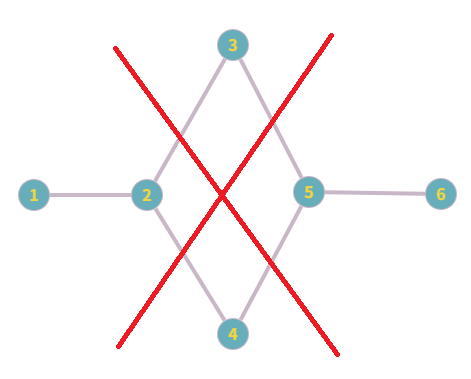
\includegraphics[height=5cm]{figures/graph006.png}}\hspace{4em}
  \subfloat[平行的一对割]{
    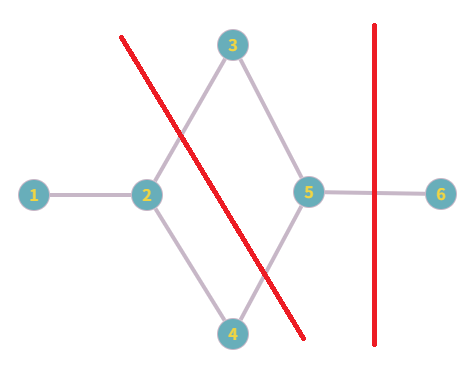
\includegraphics[height=5cm]{figures/graph007.png}}
  \caption{割的平行与相交例}
  \label{crosscut}
\end{figure}
图\ref{crosscut}给出了割相交和平行的两个例子,其中的红色直线代表一个割。

\begin{definition}[最小割图]
  给定图$G$和其最小割集$R*(G)$,最小割图按如下方式生成:
  \begin{itemize}
    \item 对于每个最小割$r*(G)\in R*(G)$,在最小割图中新建一个与之相对应的点。
    \item 若两个最小割$r_1*(G),r_2*(G)$相交,则在最小割图中对应的点之间连一条边。
  \end{itemize}
\end{definition}

\begin{lemma}[割的次模性]\cite{cunningham1985minimum}
  给定图$G=(V,E)$和图的两个割$\Delta(X),\Delta(Y)$,有
  \begin{equation*}
    w(X)+w(Y)\geq w(X\cup Y)+w(X\cap Y)
  \end{equation*}
\end{lemma}

\begin{lemma}[次模性推论]
  给定图$G$和图中两个相交的割$\Delta(X),\Delta(Y)$,则有如下结论:
  \begin{itemize}
    \item $w(X\cap Y)=\Phi_G$
    \item $w(X\cap Y,X\cap (V\backslash Y))=\frac {\Phi_G}2$
    \item $w(X\cap Y,(V\backslash X)\cap (V\backslash Y))=0$
  \end{itemize}
\end{lemma}
\begin{proof}
  根据割的次模性,我们可以得到
  \begin{equation*}
    2\Phi_G\leq w(X\cup Y)+w(X\cap Y)\leq w(X)+w(Y) = 2\Phi_G
  \end{equation*}
  因此,$w(X\cup Y)=w(X\cap Y)=\Phi_G$,第一条结论得证。

  根据第一条结论的对称性,
  $w(X\cap Y)=w(X\cap (V\backslash Y))=\Phi_G$;由于$\Delta(Y)$是最小割,所以$w(Y)=\Phi_G$。
  根据$w$的定义,有
  \begin{equation*}
    w(X\cap Y)+w(X\cap (V\backslash Y))=w(Y)+2w(X\cap Y,X\cap (V\backslash Y))
  \end{equation*}
  因此,$w(X\cap Y,X\cap (V\backslash Y))=\frac {\Phi_G}2$,第二条结论得证。

  根据第二条结论的对称性$ w(X\cap Y,X\cap (V\backslash Y))+w(X\cap Y,(V\backslash X)\cap Y)=\frac{\Phi_G}2$。
  根据$w$的定义,有
  \begin{equation*}
    w(X\cap Y,X\cap (V\backslash Y))+w(X\cap Y,(V\backslash X)\cap Y)+w(X\cap Y,(V\backslash X)\cap (V\backslash Y))=w(X\cap Y)=\Phi_G
  \end{equation*}
  因此,$w(X\cap Y,(V\backslash X)\cap (V\backslash Y))=0$,第三条结论得证。
\end{proof}

\begin{definition}[$p$割与$t$割]
  如果图$G$的一个最小割$R$与其他任何最小割都平行,我们就称它为$p$割;否则,称它为$t$割。
\end{definition}
\begin{figure}[htb]
  \centering
    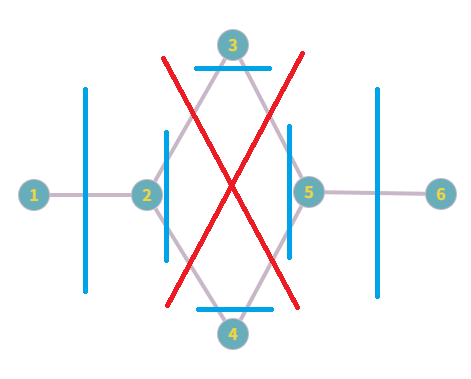
\includegraphics[height=5cm]{figures/graph008.png}
  \caption{$p$割和$t$割例}
  \label{ptcut}
\end{figure}
图\ref{ptcut}给出了图中的所有$p$割(用蓝色直线表示)和$t$割(用红色直线表示)。

\begin{definition}[处于两个$p$割之间的点和割]
  给定两个$p$割$R=(X,Y)$和$R'=(X',Y')$,
  不妨假设$X\cap Y'=\emptyset$。
  我们称点$v$处于$R$和$R'$之间当且仅当$v\in X'\cap Y$。
  我们称割$R''=(X'',Y'')$处于$R$和$R'$之间当且仅当 $X\subset X''$且$Y'\subset Y''$。
\end{definition}


\begin{figure}[htb]
  \centering
    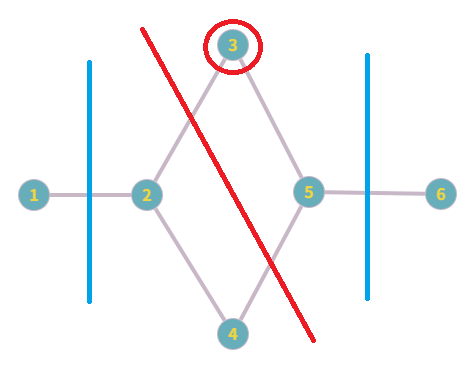
\includegraphics[height=5cm]{figures/graph009.png}
  \caption{处于两个$p$割之间的点和割例}
  \label{between}
\end{figure}
图\ref{between}中红色点以及红色代表的割处于两个蓝色直线表示的$p$割之间。

\begin{definition}[相邻的$p$割]
  给定两个$p$割$R$和$R'$,我们称它们相邻当且仅当不存在处于它们之间的$p$割。
\end{definition}
对于一个$p$割$R=(X,V\backslash X)$,我们记$S(X)$为所有与$R$相邻且分隔开$X$中顶点的割的集合。
\begin{definition}[$p$束]
  给定一个$p$割集合$S$,我们称其为$p$束当且仅当
  存在一个$p$割$R=(X,V\backslash X)$满足$S=S(X)\cup \{R\}$。
  特别的,当$S$中仅包含一个$p$割$R=(X,V\backslash X)$时,该$p$束为叶$p$束,我们用$X_S$表示,该$p$束由$R$的$X_S$一侧得到。
\end{definition}
图的所有$p$束可以通过枚举所有$p$割以及其两侧得到,也就是说,图的$p$束集合是有限且唯一确定的。

\begin{definition}[$p$束内部的顶点和$t$割]
  顶点$v$属于$p$束$S$当且仅当其在$S$中任意两个$p$割之间,$S$此类顶点的集合记作$V(S)$。
  $t$割属于$p$束$S$当且仅当其在$S$中任意两个$p$割之间。
  特别的,对于叶$p$束$S$,顶点$v$属于$S$当且仅当$v\in X_S$。
\end{definition}
这里需要特别说明的是,$t$割不会属于任何叶$p$束,这是由割的次模性推论得到的。
\begin{definition}[相邻的$p$束]
  两个$p$束$S,S'$相邻当且仅当$S\cap S'$非空。
\end{definition}
当$S,S'$相邻时,$S\cap S'$中的元素$R$是唯一的,且$S,S'$分别位于$R$的两侧。
\begin{theorem}[树表示法]\cite{dinitz1976structure}
  \label{treerepresentation}
  给定带权图$G$,存在一个棵树$\Lambda$和映射$\phi:V_G\rightarrow V_\Lambda$,满足:
    \begin{itemize}
        \item 对于点$v_1,v_2\in V_G$,$\phi(v_1)=\phi(v_2)$当且仅当图$G$不存在$p$割$R=(V_1,V_2)$使得$v_1\in V_1,v_2\in V_2$;
        \item 图$G$的最小割$R=(V_1,V_2)$与图$\Lambda$的最小割$(\phi(V_1),V_\Lambda\backslash\phi(V_1))$一一对应。
    \end{itemize}
\end{theorem}

\begin{theorem}[树表示法的性质]\cite{dinitz1976structure}
  \label{treerepresentation2}
  图$G$的树表示法$\Lambda$有以下两个性质:
  \begin{itemize}
    \item $\Lambda$上每一条边的边权都等于最小割的割值。
    \item $\Lambda$中的点与$p$束一一对应,边与$p$束的相邻关系一一对应。
  \end{itemize}
\end{theorem}

\begin{lemma}[树表示法的唯一性]
  \label{treeunique}
  给定带权图$G$,其树表示法$(\Lambda,\phi)$唯一。
\end{lemma}
\begin{proof}
  使用反证法,不妨假设图$G$有两个不相同的树表示法$(\Lambda,\phi)$和$(\Lambda',\phi')$。
  首先,根据定理\ref{treerepresentation}的第一条性质,若存在$v_1,v_2\in V_G$满足$\phi(v_1)=\phi(v_2)$但$\phi(v_1)\neq\phi(v_2)$,
  则将两点分隔开的$p$割的存在性出现矛盾。因此$\phi=\phi'$。

  图$G$的$p$束集合有限且唯一确定,而根据定理\ref{treerepresentation2}可得
  $\Lambda$中的点与$G$的$p$束一一对应,且边与$p$束的相邻关系一一对应,因此
  $\Lambda$与$\Lambda'$相同。综上,$(\Lambda,\phi)$和$(\Lambda',\phi')$是同一个树表示法。
\end{proof}


\begin{definition}[原子]
  给定图$G=(V,E)$和$G$中割的集合$\mathcal{C}$。$\mathcal{C}$的原子是一个$V$的划分$P$的所有划分块,其中$P$满足
  \begin{itemize}
    \item 对于任意割$(X,V\backslash X)\in \mathcal{C}$以及任意原子$A\in P$,满足$A\subseteq X$或$A\subseteq V\backslash X$。
    \item $P$是满足条件的最粗划分,也就是说对于任何满足条件的划分$P'$,都有$P'\preceq P$。
  \end{itemize}
\end{definition}

通俗来讲,一组割会将图的点集划分成若干个划分块,每个划分块就是一个原子。

\begin{theorem}[最小割和$p$割对应的原子集等价]\cite{dinitz1976structure}
  给定图$G$,由所有最小割构成的割集得到的原子集和由所有$p$割构成的割集得到的原子集等价。
\end{theorem}

\begin{definition}[$p$束结构图$G_S$]
定义$G_S$为图$G$中$p$束$S$的结构图,其生成方式如下:
\begin{itemize}
  \item 将$G_S$初始化为$G$。
  \item 枚举$S$中的$p$割$R$,并对被该割与$S$分隔开的点集执行点收缩(同时记收缩得到的点为$x_R$)。
\end{itemize}
\begin{definition}[$\hat c$环]
  所有边的权重都为 $\hat{c}/2$的环被称为 $\hat{c}$环。 
\end{definition}
\end{definition}
\begin{theorem}[含$t$割的$p$束的结构图为环]\cite{dinitz1976structure}
  \label{ring}
  如果一个 $p$ 束 $S$存在内部的$t$割,
  那么图 $G_S$是以顶点 $x_R$( $R\in S$)构成的 $\hat{\Phi_G}$环 。
\end{theorem}
定理\ref{ring}说明了当$p$束$S$内存在$t$割的情况,其核心结论主要有两点。第一个结论是当$S$内存在$t$割时,
则$V(S)=\emptyset$,这是由$\hat{\Phi_G}$环仅由$x_R$即$S$外部的顶点构成这一结果得到的;
第二个结论是$S$内的$t$割恰好是将环分成两部分的割(需满足每一部分至少有两个点),且这些$t$割在最小割图中恰好构成一个联通块。

通过上述定义与定理可以发现,仙人掌图表示法用非环边表示$p$割,用环边二元组表示$t$割。



\section{仙人掌图表示法的不唯一性}

考虑仙人掌图表示法中映射$\varphi$的逆映射$\varphi^{-1}$,该逆映射是从$V_\Gamma$到$\mathcal{P}(V_G)$的映射,
通俗的说,$\Gamma$中的点对应着$G$中的$0$个、$1$个或多个点。
首先,我们形式化的定义仙人掌图表示法的等价性。

\begin{definition}
  \label{cactusequal}
  给定点集$V$,仙人掌图表示法由仙人掌图$\Gamma$和映射$\varphi:V\rightarrow V_\Gamma$构成,
  其对应的割集为
  \begin{equation*}
    CutSet(\Gamma,\varphi)=\{(X,Y)\in R^*_{\Gamma}|(\bigcup_{x\in X}\varphi^{-1}(x),\bigcup_{y\in Y}\varphi^{-1}(y))\}
  \end{equation*}
  两个仙人掌图表示法$(\Gamma,\varphi),(\Gamma',\varphi')$等价当且仅当$CutSet(\Gamma,\varphi)=CutSet(\Gamma',\varphi')$。
\end{definition}

这个定义从侧面表明,一个仙人掌图表示法对应了原图的一个割集。但是,一个原图的割集可能对应多个仙人掌图表示法。

\begin{lemma}
  \label{cactusnonunique}
  图的仙人掌图表示法不具有唯一性。
\end{lemma}
\begin{proof}
  想要证明这一点,我们只需要给出一个图$G$以及其两个不相同的仙人掌图表示法$(\Gamma,\varphi),(\Gamma',\varphi')$。
  \begin{figure}[htb]
    \centering
    \subfloat[图$G$]{
      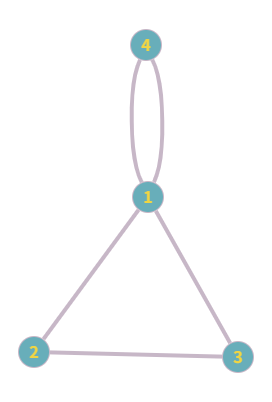
\includegraphics[height=5cm]{figures/graph003.png}}\hspace{4em}
    \subfloat[图$\Gamma$]{
        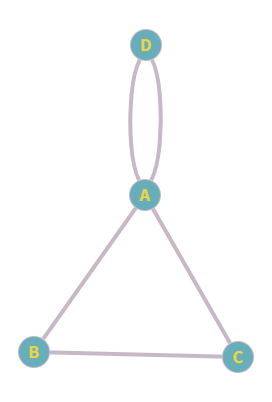
\includegraphics[height=5cm]{figures/graph004.png}}\hspace{4em}
    \subfloat[图$\Gamma'$]{
      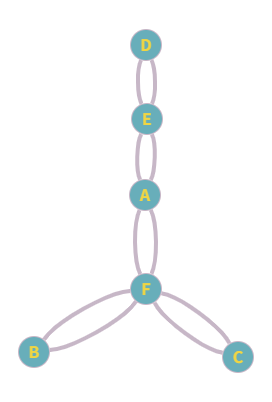
\includegraphics[height=5cm]{figures/graph005.png}}
    \caption{同一个图的两种仙人掌图表示法}
\end{figure}

我们给出了一个$n=4$的例子,$G,\Gamma,\Gamma'$的结构如图所示,且映射满足
\begin{equation*}
  \varphi=\varphi'=\{(1,A),(2,B),(3,C),(4,D)\}
\end{equation*}
在这个例子中,原图的最小割有$(\{1,4\},\{2,3\}),(\{1,2,4\},\{3\}),(\{1,3,4\},\{2\}),(\{1,2,3\},\{4\})$。
仙人掌图表示法$(\Gamma,\varphi)$使用了与图$G$相同的结构,因此其最小割与原图的最小割一一对应。
仙人掌图表示法$(\Gamma',\varphi')$进行了两个改动:
第一个改动是通过加入节点$F$,使$A,B,C$构成的三元环变成三个二元环,
三元环所表示的最小割分别转而由这三个二元环所表示,所以该改动不影响割集
以割$(\{1,3,4\},\{2\})$为例,其由$\Gamma$中的三元环边$(A,B),(B,C)$共同表示,
而到了$\Gamma'$中,其转而由两条$(B,F)$边构成的二元环表示;
第二个改动是在$A$和$D$之间加入$E$,这使得$\Gamma'$中的最小割数量增加,
即$(\{A,B,C,F\},\{D\})$扩展成了$(\{A,B,C,F\},\{D,E\})$和$(\{A,B,C,E,F\},\{D\})$两个最小割,
然而由于$\varphi^{-1}(E)=\emptyset$,因此这两个$\Gamma'$中的割对应$G$的同一个割,改动不影响割集。
综上,$(\Gamma,\varphi),(\Gamma',\varphi')$都是$G$的仙人掌图表示法,图的仙人掌图表示法不具有唯一性。
\end{proof}

虽然图的仙人掌图表示法不具有唯一性,但其仙人掌图表示法相互等价,
这是由表示的最小割集的唯一性得出的。
因此,如果在仙人掌图表示法的生成算法中加入仙人掌图表示法的标准化算法$ALG_{std}$,
将输出的仙人掌图表示法转化为其等价类的标准元,
那么就可以确保算法输出的唯一性。

特别的,仙人掌图表示法的标准化在差分隐私下尤为重要。
对于最小割集相同的边相邻图,算法得到的仙人掌图表示法可能因边集的差异而不同,
而在标准化处理后,输出将正确地被判定为相同。

\section{标准化仙人掌图表示法}

本节中,仙人掌图表示法的标准化共分为两部分。
第一步是通过给出构造方法定义仙人掌图表示法的标准元。
第二步是给出将现有仙人掌图表示法转化为其标准元的高效算法。

根据引理\ref{treeunique},树表示法$\Lambda$可以表示所有$p$割且方法唯一。
根据定理\ref{ring},$p$束的结构图可以表示该$p$束的所有$t$割且方法唯一。
因此,如果将树表示法和每个$p$束的结构图进行合成得到的图也是唯一的,且恰好能表示所有的最小割,
我们将这个图设置为该仙人掌图表示法的标准元。
算法\ref{alg:gen}给出了$ALG_{gen}$的具体实现。我们称$ALG_gen(G)$为图$G$的标准仙人掌图表示法。

\begin{algorithm}
  \caption{图$G$的仙人掌图表示法构造算法$ALG_{gen}$}
  \label{alg:gen}
  \begin{algorithmic}[1] % [1] 表示从第1行开始编号
  \Statex 输入:图$G$
  \Statex 输出:仙人掌图表示法$(\Gamma,\varphi)$
  \State 计算图$G$的$p$割,$t$割。
  \State 计算图$G$中的所有$p$束。
  \State 为每个$p$束$S$新建一个$\Gamma$中的点$v_S$,并更新$S$内的点到$v_S$的映射$\varphi$。
  \State 若两个$p$束$S,S'$相邻,则为其在$\Gamma$中的点$v_S,v_{S'}$连一条边,得到图$G$的树表示法。
  \State 若$p$束$S$中有$t$割,则将$v_S$替换为$G_S$,原本连向$v_S$的代表$p$割$R$的边重新连向$G_S$中的点$x_R$。
  \State \Return $(\Gamma,\varphi)$
  \end{algorithmic}
\end{algorithm}

\begin{theorem}
  给定图$G,G'$,其仙人掌图表示法分别为$(\Gamma,\varphi)$和$(\Gamma',\varphi')$。
  若$(\Gamma,\varphi)$和$(\Gamma',\varphi')$等价,则$ALG_{gen}(G)=ALG_{gen}(G')$
\end{theorem}

\begin{proof}
  $(\Gamma,\varphi)$和$(\Gamma',\varphi')$等价,则根据定义\ref{cactusequal},有 $CutSet(\Gamma,\varphi)=CutSet(\Gamma',\varphi')$。
  由仙人掌图表示法的定义,
  $CutSet(\Gamma,\varphi)$和$CutSet(\Gamma',\varphi')$分别对应$\Gamma$的最小割集和$\Gamma'$的最小割集。
  $ALG_{gen}(G)$的仅与$G$的最小割集有关,因此$ALG_{gen}(G)=ALG_{gen}(G')$。

\end{proof}

算法$ALG_{gen}(G)$给出了仙人掌图表示法的标准元,但难以直接用于仙人掌图表示法构造算法中。
因为算法没有提供一个高效的计算方法,而朴素的$p$割,$t$割,$p$束计算需要较高复杂度,继而成为算法的效率瓶颈。

我们发现,如果我们首先利用现有工作生成一个仙人掌图表示法,然后使用仙人掌图表示法标准化算法$ALG_{std}$,
将仙人掌图表示法转化为其等价类内的标准元,那么就能同时实现高效和标准化。
与此同时,$ALG_{std}$可以通过输入仙人掌图表示法本身的性质,来得到一个较好的复杂度。


\begin{algorithm}
  \caption{仙人掌图表示法标准化算法$ALG_{std}$}
  \label{algstd}
  \begin{algorithmic}[1] % [1] 表示从第1行开始编号
  \Statex 输入:仙人掌图表示法$(\Gamma,\varphi)$
  \Statex 输出:仙人掌图表示法$(\Gamma',\varphi')$
  \State 设仙人掌图表示法$(\Gamma,\varphi)$的最小割的割值为$c$
  \State 对于所有二元环,将环上的两条边合并为一条边。\Comment{二元环表示$p$割}
  \For {$\Gamma$中的简单环$C$}
      \For {$C$中的节点$k$}
          \State 在$\Gamma$中新建顶点$k',k''$来替换$k$
          \State 令$\varphi^{-1}(k'')=\varphi^{-1}(k),\varphi^{-1}(k')=\emptyset$
          \State 在$k',k''$之间连一条边权为$c$的边
          \For {与$k$相连的边$e$}
            \If{$e$是环$C$上的边}
                \State 将$e$的$k$一端替换成$k'$
            \ElsIf{$e$是环$C$上的边}
                \State 将$e$的$k$一端替换成$k''$
            \EndIf
          \EndFor
      \EndFor
  \EndFor
  \State 对$\Gamma$中的所有三元环执行点收缩。\Comment{三元环只表示$p$割}
  \For {$\Gamma$中度数为$2$的点$v$}
      \State 找到与$v$相连的边$(v,u_1),(v,u_2)$
      \If{若$v$不处于任何一个简单环上且$\varphi^{-1}(v)=\emptyset$}
          \State 删除点$v$以及与其相连的边
          \State 加入边$(u_1,u_2)$
      \EndIf
  \EndFor
  \State \Return $(\Gamma',\varphi')$
  \end{algorithmic}
\end{algorithm}

回顾引理\ref{cactusnonunique}中的例子,仙人掌图表示法主要需要解决的是三元环和链两种情况。
算法\ref{algstd}给出了$ALG_{std}$的具体实现。

\begin{theorem}
  给定图$G$和其仙人掌图表示法$(\Gamma,\varphi)$,则$ALG_{std}((\Gamma,\varphi))=ALG_{gen}(G)$
\end{theorem}

\begin{proof}
  首先,我们分析仙人掌图表示中,单个环表示的最小割的数量和类型。根据定理\ref{ring}

  首先,我们需要证明$ALG_{std}((\Gamma,\varphi))$算法得到的环与$ALG_{gen}(G)$的环一一对应。
  在仙人掌图表示中,非环边代表的最小割一定是$p$割,环中代表的最小割可能有$p$割也可能有$t$割。
  根据算法\ref{alg:gen}可知,$ALG_{gen}(G)$的环仅用于表示$t$割。对于一个$ALG_{gen}(G)$里的简单环$C$,
  若其表示的$t$割在最小割图中恰好构成一个连通块,因此这些割在$(\Gamma,\varphi)$中
  一定由一个相同的环$C'$表示。对于一个仙人掌图表示$(\Gamma,\varphi)$中的环$C'$,环上相邻的两条边可以表示一个$p$割,
  这些$p$割在算法中通过$(k',k'')$这条非环边重新表示了;
  若环$C'$不表示任何$t$割,那么其一定是一个二元环或三元环,在算法中被消除。
  综上,$ALG_{std}((\Gamma,\varphi))$算法得到的环与$ALG_{gen}(G)$的环一一对应。

  接下来,我们证明将所有环缩成点后,
  $ALG_{std}((\Gamma,\varphi))$的树结构和$ALG_{gen}(G)$的树结构相同。
  $(\Gamma,\varphi)$的$p$割由非环边和环共同表示,而在处理环的过程中,
  所有环表示的$p$割转而以$(k',k'')$的形式表示。因此,处理完环之后,$(\Gamma,\varphi)$的树结构和$ALG_{gen}(G)$
  都能表示所有$p$割。$(\Gamma,\varphi)$的树结构表示了所有$p$割,但不一定是树表示法,
  因为树表示法的边与$p$割一一对应,但是树结构可以存在多条边对应同一个$p$割。
  由于代表同一个$p$割的两条边之间的树上路径的点$v$都满足$\varphi^{-1}=\emptyset$,
  因此,$ALG_{std}$通过收缩这样的点,就可将树结构转化为树表示法。
  根据定理\ref{treerepresentation},树表示法具有唯一性。
  综上, $ALG_{std}((\Gamma,\varphi))$的树结构和$ALG_{gen}(G)$的树结构相同。

  最终,结合以上两个结果,可以得出$ALG_{std}((\Gamma,\varphi))=ALG_{gen}(G)$。
\end{proof}

\chapter{最小割数量的敏感度分析}
\section{最小割数量的敏感度}
在求解近似最小割的过程中,需要尽可能找到多的解,
然而差分隐私的算法要求一条边的存在与否对输出的影响不能过大。
因此,需要首先对最小割数量进行敏感性进行定量分析,
才能设计出恰当的噪声添加值。

假设现在有两个边相邻的图$G,G'$,其中$G'$由在$G$中加入一条边权为$1$的边$(u,v)$得到。
不妨假设最小割数量计算函数的输入与输出都以适当的二进制形式进行编码,
可以得到最小割数量的敏感度为$d=|M_G-M_{G'}|$。

我们知道,对于任意图$G$,最小割数量满足$1\leq M_G\leq n^2$,因此$0\leq d\leq n^2$。


\begin{lemma}
  \label{lemma:mingganN}
  对于任意$n\geq 3$,存在图$G,G'$的构造方法,使得最小割数量的敏感度为$\Omega(n^2)$。
\end{lemma}
\begin{proof}
  我们不妨将点集中的点编号,用$v_1$至$v_n$表示。下面给出构造方法:
  图$G$由如下方法生成,连接$v_1$与$v_2$,$v_2$与$v_n$,并对于所有整数$2\leq i<n$,连接$v_i$和$v_{i+1}$;
  图$G'$由图$G$的基础上,增加一条连接$v_1$和$v_2$的边得到。
  
  这里的连边均为$1$,因此图$G$的最小割值为$1$,唯一的方案是$(\{v_1\},V\backslash v_1)$,因此$M_G=1$。
  图$G'$的最小割值为$2$,此时对于任意$2\leq i\leq j\leq n$,
  $(\{v_i,\ldots,v_j\},V\backslash \{v_i,\ldots,v_j\})$都是一个最小割,
  因此$M_{G'}=\frac{n^2-n}2$。在这种构造方法下,$d=\Omega(n^2)$。
\end{proof}
\begin{figure}[htb]
    \centering
    \subfloat[图$G$]{
      \label{1}
      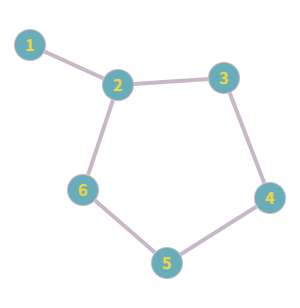
\includegraphics[height=5cm]{figures/graph001.png}}\hspace{4em}
    \subfloat[图$G'$]{
      \label{2}
      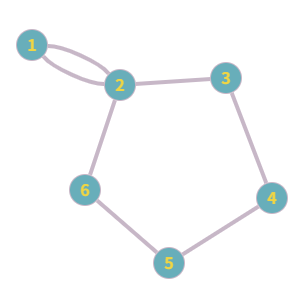
\includegraphics[height=5cm]{figures/graph002.png}}
    \caption{$n=6$时的构造示例}
    \label{fig:exA}
\end{figure}
图\ref{fig:exA}给出了一种$n=6$时的构造示例。
引理表明,边相邻图的最小割数量的敏感度在一些情况下特别高,
高敏感度意味着需要添加较大噪声,进而使得差分隐私下发布的最小割数量可用性较低。
因此在设计算法时,需要引入一些额外的约束条件。
\section{约束条件下的敏感度}
给定图$G$,在加入一条单位边后,最小割的割值可能增加,也可能保持不变。
引理\ref{lemma:mingganN}指出,若图有一个割值为$x$的割和较多割值为$x+1$的割,
那么加边导致最小割的割值提高$1$后,会使最小割的数量出现较大的增幅。
因此,为了得到可用的结果,可以加入边相邻图的最小割值相同这一额外限制条件,
也就是说,图$G,G'$满足$\Phi_G=\Phi_{G'}$。在本章的后文中,如未特殊说明,图$G,G'$将默认满足这一性质。


标准仙人掌图表示法包含了图所有最小割的信息,因此其结构参数有助于对问题分析的精细性。所以,
对于一个图$G$以及其标准仙人掌图表示法$(\Gamma,\varphi)$,我们引入以下参数来描述图的结构:
\begin{itemize}
  % \item $\alpha_{n}$:图$G$的点数,即$|V_G|$%平均用的吧
  \item $\alpha_{g}$:标准仙人掌图表示法的点数,即$|V_{\Gamma}|$。
  \item $\alpha_{p}$:标准仙人掌图表示中所有点$v$对应的$|\varphi^{-1}(v)|$的最大值%平均用的吧
  \item $\alpha_{c}$:标准仙人掌图表示中环的数量。
  \item $\alpha_{r}$:标准仙人掌图表示中环长度的最大值。
  \item $\alpha_{d}$:标准仙人掌图表示中树结构的直径,也就是所有图上简单路径中,非环边数量的最大值。
  % \item $\beta_{p}$:图$G$的$p$割数量。
  % \item $\beta_{t}$:图$G$的$t$割数量。
\end{itemize}


在$G$中加入一条边权为$1$的边$(u,v)$得到$G'$,
接下来我们分析这条边$(u,v)$在标准仙人掌图表示法$(\Gamma,\varphi)$中的位置与最小割数量变化量的关系。
首先,若$\varphi(u)=\varphi(v)$,那么说明$u,v$之间不被任何最小割分隔开,
在仙人掌图表示法中它们已经被视为连通性很高的两个点,因此加入边$(u,v)$对最小割数量没有任何影响。

若$\varphi(u)\neq\varphi(v)$,我们不妨令$U=\varphi(u)$,$V=\varphi(V)$。
根据标准仙人掌图表示法的构造过程可知,其表示最小割的结构主要有树表示和每个$p$束对应的结构环两部分。
树表示中$U$到$V$路径上的所有$p$割都将不再是最小割,路径上所有$p$束对应的结构环代表的$t$割都会变少。
具体来说,对于一个$p$束$S$的结构环$G_S$,令$U\in x_{R'},V\in x_{R''}$,
所有将$x_{R'}$与$x_{R''}$分开的$t$割都将不再是最小割。

接下来对环上的情况进行定量分析。令$f(x)$为长度为$x$的环表示的$t$割数量,则
\begin{equation*}
  f(x)=\begin{cases}
    \frac{x(x-3)}2&x\geq 3\\0&1\leq x\leq 2\end{cases}  
\end{equation*}
假设结构环$G_S$的环长为$l$,$x_{R'}$与$x_{R''}$在环上的距离为$t$(满足$t\leq l-t$),
那么最小割的减少量为
\begin{equation*}
  g(l,t)=f(l)-f(t)-f(l-t)-[t\geq 3]-[l-t\geq 3]
\end{equation*}
令$G(l)=\max_{t=1}^{l-1}g(l,t)$,我们不妨对$l,t$的值进行讨论来得到该函数的取值:
当$1\leq l\leq 3$时,环上不包含$t$割,因此$G(l)=0$;
当$l=4$时,取$t=2$为极值,$G(4)=2$;
当$l\geq 5$时,由于$l-t\geq t$,且$f$为单调函数
因此我们只需要讨论$t=2,t\geq 3$这两种情况。
\begin{itemize}
  \item 当$t=2$时,$g(l,2)=f(l)-f(l-2)-1=2l-6$;
  \item 当$t\geq 3$时,$g(l,t)=f(l)-f(t)-f(l-t)-2=-(t-\frac l2)^2+\frac{l^2}4-2$。
\end{itemize}
当$l=5$时,$t\leq 2$,因此$G(5)=g(5,2)=4$。
当$l\geq 6$时,$g(l,t)$的极小值在$t=\left\lfloor\frac l2\right\rfloor$时取到,
此时$g(l,t)\geq g(l,2)$。综上,可以得到
\begin{equation*}
  G(l)=\max{\{0,\lfloor\frac{l^2}4-2\rfloor\}}
\end{equation*}

除此之外,可以发现,加入$(u,v)$使最小割的割值增加一的情况只有在$\varphi(u)\neq\varphi(v)$,
标准仙人掌图表示法中的树表示是一条链,且$\varphi(u),\varphi(v)$分别是链的两个端点时出现。

接下来,我们给出最小割数量变化范围的表达式。

\begin{theorem}
    给定边相邻图$G,G'$,其中$G'$由在$G$中加入一条边权为$1$的边$(u,v)$得到。那么有
    \begin{equation*}
      M_G-\min{\{\alpha_d,\alpha_c,\frac{\alpha_g}{\alpha_r}\}}·\max{\{0,\lfloor\frac{\alpha_r^2}4-2\rfloor\}}-\alpha_d \leq M_{G'}\leq M_G
    \end{equation*}

\end{theorem}

最小割数量的变化还可以由$M_G$本身的值进行估计。
对于一个长度$l\geq 4$的环$G_S$,其表示的$t$割有$f(l)=\frac{l(l-3)}2$个,
边$(u,v)$经过它是会使其最小割数量减少至多$G(l)= \lfloor\frac{l^2}4-2\rfloor$。
此外不难证明,该$p$束$S$连接的不涉及$x_{R'},x_{R''}$的至少$l-2$条边对应的$p$割在加边后仍然为最小割。
因此,与该$p$束$S$相关的最小割的数量为$\frac{l^2-l-4}2$,减少量至多为$\lfloor\frac{l^2}4-2\rfloor$。
\begin{theorem}
  对于任意加边$(u,v)$,存在一种最小割分配方案,满足每个最小割至多分配至一个$p$束中,使得
  每个$p$束$S$损失的最小割数量不超过其分配量与$|G_S|$和的一半。
\end{theorem}

\begin{proof}
  按上文方法分配最小割后,$p$束$S$分配到的最小割数量为$\frac{l^2-l-4}2$,$G_S=l$
  其损失的最小割数量为$\lfloor\frac{l^2}4-2\rfloor$。有
  \begin{equation*}
    \frac{l^2-l-4}2+l=\frac{l^2+l-4}2\geq \frac{l^2}2-4\geq 2\lfloor\frac{l^2}4-2\rfloor
  \end{equation*}
\end{proof}
因此我们可以给出基于$M_G$的估计。

% 我们再给出最小割数量的估计
% \begin{theorem}
%   给定图$G$,有
%   \begin{equation*}
%     \max{\{0,\frac{\alpha_r(\alpha_r-3)}2\}}+\alpha_d\leq M_G\leq \min{\{\alpha_c,\frac{\alpha_g}{\alpha_r}\}}·\max{\{0,\frac{\alpha_r(\alpha_r-3)}2\}}+\alpha_d
%   \end{equation*}

% \end{theorem}
\begin{theorem}
  \label{sen}
  给定边相邻图$G,G'$,其中$G'$由在$G$中加入一条边权为$1$的边$(u,v)$得到。那么有
  \begin{equation*}
    \frac{M_G}2-1.5n \leq M_{G'}\leq M_G
  \end{equation*}

\end{theorem}
该定理给出了最小割数量敏感度的上界$\frac{M_G}2+1.5n$。
接下来将给出一个构造来说明这个上界可以近似的达到,
该构造下的最小割数量的敏感度与定理中最坏情况下的敏感度仅相差一个常乘法系数,
图$G$构造方法如下:
将$(1-\alpha) n$的点用边权$c$连成一条链,设链的两端分别为$v_1,v_2$;
将$\alpha n\geq 4$的点用边权$\frac c2$连成一个环,设环的一个对角线连接的两个点为$v_3,v_4$;
最后将$v_2,v_3$用边权为$c$的边相连,完成构造。

首先,$M_G=n+\frac{\alpha n(\alpha n-3)}2$。敏感度最高的加边是$(v_1,v_4)$,
敏感度$M_G-M_{G'}=\lfloor\frac{\alpha^2 n^2}4\rfloor+(1-\alpha) n$。
不失一般性地取$\alpha=\frac 12$,可得$M_G=\frac{n(n+2)}8$,$M_G-M_{G'}=\lfloor\frac{n^2}{16}\rfloor+\frac 12n$。
此时有
\begin{equation*}
  \frac{M_G}2+\frac32n= \frac{n^2}{16}+\frac{13}{8}n\leq 4(M_G-M_{G'})
\end{equation*}


\section{平均敏感度}
前面的分析表明,在最坏情况下,最小割数量的敏感度较高。这一小节将通过平均敏感度分析造成高敏感度的情况的频次。

在平均敏感性的通常定义中,其边相邻的图以删边的形式给出。\cite{varma2023average}
然而在前文描述边相邻图时,由于删边会较大的改变仙人掌表示的结构,因此用加边的形式描述了$G,G'$间的关系。
这一部分将沿用加边的方法来定义平均敏感度。
通过删边形式的平均敏感度,可以估计一个图算法在规模较大的子图上的输出和完整图上的输出差异,
改为加边形式会弱化这一功能。加边形式的平均敏感度能对应前文的分析,并给出最小割数量变化值的期望。

\begin{definition}
  图算法$A$的平均敏感度为
  \begin{equation*}
    \mathbb E_{e\in V^2,\Phi(G)=\Phi((V,E\cup\{e\}))}[d_{Ham}(A(G),A((V,E\cup\{e\})))]
  \end{equation*}
\end{definition}

考虑这样一种$G$的构造,生成一个规模为$\frac 13n$的图$G_t$,
使得$G_t$在加入边$(u,v)$时得到该规模下最高的敏感度$W(\frac 13n)$,
接下来将$\frac 13n$个点与$u$用极大的边权相连,将$\frac 13n$个点与$v$用极大的边权相连。
此时最小割数量函数$M$的平均敏感度满足
\begin{equation*}
  \mathbb E_{e\in V^2,\Phi(G)=\Phi(G+e)}[d_{Ham}(M(G),M(G+e))]\geq \frac{\frac 13n(\frac 13n-1)}{n(n-1)}W(\frac 13n)
\end{equation*}
最高敏感度$W$是一个$n$的不超过二次的一个多项式。综上,存在一个常数$\beta$使得在该构造下
\begin{equation*}
  \mathbb E_{e\in V^2,\Phi(G)=\Phi(G+e)}[d_{Ham}(M(G),M(G+e))]\geq \beta W(n)
\end{equation*}
分析表明,在最坏情况下,导致高敏感度的加边出现频率的期望较高。

\chapter{差分隐私背景下近似最小割求解算法}

本章将详细阐述差分隐私背景下近似最小割求解算法的具体设计方案。
该算法不仅需满足差分隐私的要求,同时要有效控制近似最小割与真实最小割之间的加法误差;
此外,算法还需尽可能多地输出有效的近似最小割的解,并兼顾算法的运行效率。
形式化的来说,算法的输入为图$G$,给定隐私参数$\varepsilon,\delta$和误差$\Delta$,
算法应当能$(\varepsilon,\delta)$-差分隐私地输出一个尽可能大的割集$R$,使得对于任意割$r\in R$,
满足$w(r)\leq \Phi_G+\Delta$。

\section{基于差分隐私图的算法设计}

算法设计的难点在于,输入的数据需要隐私化处理后才能使用。
对图直接进行差分隐私是一种可行的方案,且在隐私化后的图上进行计算可以使用非差分隐私算法。
定理\ref{the:dpgraph}展示了Liu等人设计的差分隐私图算法。
回顾该算法内容,
对于一个输入$G$,算法可以以高概率$(\varepsilon,\delta)$-差分隐私地输出一个合成图$\hat G$。
对于合成图中任意不相交的点集$ S, T \subseteq V_G $,均满足如下关系
    \begin{equation}
        |w_G(S, T) - w_{\hat{G}}(S, T)| = O\left(\frac{\sqrt{nm}}{\varepsilon} \log^3 \left(\frac{n}{\delta}\right)\right)   
    \end{equation}
这表明,对于原图中的任意最小割$R$,其在合成图$\hat G$中的割值为$\Phi_G+ O\left(\frac{\sqrt{nm}}{\varepsilon} \log^3 \left(\frac{n}{\delta}\right)\right)$。
由此可见,合成图$\hat G$作为图$G$隐私处理后的结果,能够确保最小割有较好的近似,
也就是说,该方法能确保合成图中的近似最小割数量不少于原图的最小割数量。

在完成图的隐私化步骤后,算法可以枚举合成图中的所有割,并将割值与$\Phi_G+\Delta$比较。
因此,算法需要差分隐私地发布最小割割值$\Phi_G$,即得到一个误差较小的近似值$\hat \Phi_G$,
这一任务可以由拉普拉斯机制完成。

差分隐私地计算最小割值的方法如下:
首先,使用定理\ref{the:mincut}中的Karger最小割算法,
可以以高概率求出图$G$的最小割值$\Phi_G$。
在边相邻的两个图$G,G'$中,恰好存在一条边边权相差$1$,其它边边权均相等,
因此,图$G$中的一个最小割在图$G'$中的割值最多增加一。
根据定理\ref{laplace}中的拉普拉斯机制,
将最小割值作为函数$f$,则其对应的敏感度$\Delta=1$,
因此对最小割的真实加入噪声后,
算法能以$\varepsilon$-差分隐私的发布最小割值的近似值$\hat \Phi_G=\Phi_G+X$,
其中$X\sim Lap(1/\varepsilon)$。

使用拉普拉斯机制带来的误差为$O(\frac{1}{\varepsilon})$。
具体分析如下:拉普拉斯分布$Lap(1/\varepsilon)$的概率密度函数为
\begin{equation}
    f(x)=\frac \varepsilon{2} e^{-\varepsilon\|x\|}
\end{equation}
对$x$取绝对值后,函数变成指数分布的形式,其概率密度函数为
\begin{equation}
    f(x)=\varepsilon e^{-\varepsilon x},(x\geq 0)
\end{equation}
绝对值的累计分布函数为
\begin{equation}
    P(|X|\leq t)=1-e^{-\varepsilon x},(t\geq 0)
\end{equation}
由该式可得,有至少$1-\alpha$的概率使得
$|X|\leq \frac1\varepsilon\ln\left(\frac1\alpha\right)$。
因此,算法有高概率满足$\hat\Phi(G)=\Phi(G)+O(\frac1\varepsilon)$。

在差分隐私地求得最小割的近似值后,算法可以通过枚举割并对割值进行判断来求得解。
具体来说,算法将$\beta$定为一个足够大的常数,并枚举$V_G$的所有子集$X$,
判断$\Delta(X)$在合成图$\hat G$中的割值是否满足
$w_{\hat G}(X)\leq \hat \Phi_G+\beta \frac{\sqrt{nm}}{\varepsilon} \log^3 \left(\frac{n}{\delta}\right)$,
满足条件的$\Delta(X)$被视为近似最小割并加入输出的割集$R$中。
需要注意的是,输出的割集$R$会包含图$G$中的所有最小割和部分近似最小割,
因此割集$R$的大小可能超过$n^2$。

使用定理\ref{the:basic}这一基本组合定理,
可以为算法中差分隐私步骤的$\epsilon$和$\delta$赋合适的常系数,
不难说明,
上述算法是$(\varepsilon,\delta)$-差分隐私的,
且能以高概率输出至少$M_G$个
$O\left(\frac{\sqrt{nm}\log^3 \left(\frac{n}{\delta}\right)}{\varepsilon} \right)$近似的最小割。

\section{基于$k$优选择机制的算法设计}

除了对图直接进行隐私化处理外,算法也可以在对原图进行若干计算后再进行差分隐私。
定理\ref{the:topk}中提到的$k$优选择机制可以$(\varepsilon,\delta)$-差分隐私地
在$m$个值中取$k$个$O(\frac{\sqrt{k\log(m/\delta)}}{\varepsilon})$近似最小值。
因此,算法可以差分隐私的获取最小割值$\hat \Phi_G$和最小割的数量$\hat M_G$,
并用$k$优选择机制在所有$2^n$个割中选择权值前$\hat M_G$小的割。
通过该方法,算法可以获得$\hat M_G$个割,再进行筛选处理可以得到差分隐私背景下的近似最小割。

回顾最小割数量的敏感度,根据定理\ref{sen},给定边相邻图$G,G'$,
其中$G'$由在$G$中加入一条边权为$1$的边得到,则有
$0\leq M_G-M_{G'}\leq \frac{M_G}2+1.5n$。
由于边相邻图的最小割数量较大,因此需要取对数处理。
不妨令$a=\log_2(M_G+3n)$,其敏感度为$1$。
接下来,使用拉普拉斯机制差分隐私的输出$a$的值$\hat a$,
并令差分隐私的最小割数量为$\hat M_G=min{\{max{\{0,2^{\hat a}-3n\}},n^2\}}$。

得到估计值$\hat\Phi_G$和$\hat M_G$后,
算法可以枚举$V_G$的所有子集$X$,
并计算割$\Delta(X)$在原图$G$中的割值。
对所有$2^n$个割值使用定理\ref{the:topk}中的$k$优选择机制,
算法可以得到$\hat M_G$个割
以及每个割的$O(\frac{n\sqrt{n\log(1/\delta)}}{\varepsilon})$近似值。
由于对最小割数量的估计存在误差,因此原图的第$\hat M_G$小割可能并非最小割,
因此,筛选处理在本节的算法仍然是必要的。
与上一节类似,
算法将$\beta$定为一个足够大的常数,
并枚举所有这$\hat M_G$个割,并分别判断其割值是否小于
$\hat \Phi_G+\beta \frac{n\sqrt{n\log(1/\delta)}}{\varepsilon}$,
满足条件的割视被视为近似最小割并加入输出的割集$R$中。

相比于基于差分隐私图的算法,该算法加入了对最小割数量的估计,
因此适用于要求输出割数量与原图$G$中最小割数量相仿时的场景。
然而,本文中给出的差分隐私的最小割数量估计算法误差较大,
算法可能出现输出割集大小远小于原图$G$中最小割数量的问题,这与目标相悖。

为了解决$\hat M_G$过小的情况,算法需要进行一些修改。
对于图$G$的$M_G$个最小割中的每个割,其在$k$优选择机制中的的割值为$\Phi_G+O(\frac{\sqrt{kn\log(1/\delta)}}{\varepsilon})$。
$\hat M_G$的规模为$O(n^2)$,因此代入$k$的取值后,
可以保证原图$G$的最小割在筛选步骤中不会被排除在外。
因此当$\hat M_G\leq M_G$时,$k$优选择机制得到的割一定不会在筛选步骤中被排除在外。
由于筛选机制的存在,可以令$k=n^2\geq M_G$,
这样能保证输出的近似最小割数量不少于原图最小割的数量。

修改后的基于$k$优选择机制的算法的表现并不比基于差分隐私图的算法更好,
但其提供了一种对原图进行进一步处理以实现算法优化的可能性。

\section{加法近似参数的优化}

当$m=\Theta (n^2)$时,
基于差分隐私图的算法与基于$k$优选择机制的算法,
其加法近似参数均为$\tilde O(\frac{n\sqrt n}{\varepsilon})$。
本节提出一种融合指数机制与Karger收缩算法的方法,旨在降低加法近似参数。

回顾$k$优选择机制,算法从$m$个数中选择了$k$个最小值,
其加法近似参数$O(\frac{\sqrt{k\log(m/\delta)}}{\varepsilon})$同时由$m,k$决定。
而受到最小割数量的限制,在最坏情况下,$k$的取值为$\Theta (n^2)$。
因此要想优化加法近似参数,需要从降低$m$入手。

在上一节中,算法枚举了点集的所有子集来寻找割,
这是因为在没有给定更多条件的情况下,
图中所有割都是潜在的$k$小割,因此$m=2^n$。
算法需要缩小潜在$k$小割的范围来使$m$值降低。

由于$k$的值为$O(n^2)$,因此$k$小割可以视为原图的一个近似最小割。
前文提到,当$\alpha$为一常数时,
Karger收缩算法可以在多项式复杂度内找到所有$\alpha$乘法近似最小割。
具体来说,根据定理\ref{the:agl},一个给定的$\alpha$乘法近似最小割在收缩至$\lfloor2\alpha\rfloor$个顶点时,
其有效的概率为$\Omega(n^{-2\alpha})$。因此,执行$n^{2\alpha+1}$次Karger收缩算法,
则该$\alpha$乘法近似最小割以高概率在至少一次算法执行中有效。因此,以高概率所有$\alpha$乘法近似最小割都被找到。
Karger收缩算法本身为非差分隐私算法,
因此在处理其输入时需要考虑隐私性。


设调用$k$优选择机制时算法的加法近似参数为$\Delta'$,
则应有$\Delta'\leq \Delta$。
若如此,则对于图$G$的任意最小割,
在调用$k$优选择机制时割值均小于$\Phi_G+\Delta$,
则可保证找到的近似最小割数量不少于原图的最小割数量。

Karger收缩算法可以找到割值不超过$\alpha\Phi_G$的所有割,
而本文提出的算法需要寻找割值不超过$\Phi_G+\Delta'$的最小割。
前者采用乘法近似参数,后者采用加法近似参数,
参数形式的差异要求对算法进行额外分析。
联立两式得$\alpha=1+\frac {\Delta'}{\Phi_G}$,
由于Karger收缩算法求得的近似最小割数量与$\alpha$有关,
因此$\alpha$的值需取为常数。
也就是说,算法需要对$G$进行一定处理来保证$\frac {\Delta'}{\Phi_G}$存在一个常数上界。

对$G$的处理应该在引入较少误差$\Delta'$的同时,
又能提高最小割的割值。
具体方法为在图$G=(V,E)$中差分隐私地加边加边。
算法使用指数分布来差分隐私地选择加边的边集。
首先给定参数$T$,算法按如下方法构造一个边集$H$:
\begin{itemize}
    \item 将图$G$的$n$个顶点按任意顺序排列成一个环。
    \item 对环上任意相邻两点,在$H$中加入$T/2$条连接这两个点的边权为$1$的边。
\end{itemize}
接下来,令$H_0\subset H_1,\ldots,\subset H_{|H|}$为任意大小严格递增的边集序列,且$H_{|H|}=H$。
对于每个下标$i\in[1,|H|]$,令其权值为$t_i=|\Phi_{(V,E\cup H_i)}-T|$。
使用指数机制选择下标$i$,则有高概率得到一个解,满足
\begin{equation}
    Pr[|\Phi_{(V,E\cup H_i)}-T|>t_{min}+\frac{2\ln (nT)}{\varepsilon}+\frac{2t}{\varepsilon}]\leq e^{-t}
\end{equation}
容易证明,$t_{min}=\max\{0,\Phi_G-T\}$。
令$T=\frac{20\ln n}{\varepsilon}$,令$t=2\ln n$。
整理,记
\begin{equation}
    t_{range}=\frac{2\ln (nT)}{\varepsilon}+\frac{2t}{\varepsilon}=\frac{6\ln n+2\ln T}{\varepsilon}= \frac{6\ln n+2\ln(20\ln n)-2\ln \varepsilon}{\varepsilon}
\end{equation}
当$\varepsilon\in[\frac1n,\frac12]$,$n\geq 200$时,有$t_{range}\leq \frac{10\ln n}{\varepsilon}$。

记$\hat G=(V,E\cup H_i)$,讨论$\Phi_G$与$T$的关系并化简,可以得出算法以$1-\frac1{n^2}$的概率满足
\begin{equation}
    10\ln n/\varepsilon<\Phi_{\hat G}<\Phi_G+30\ln n/\varepsilon
\end{equation}

在上述生成$\hat G$的过程中,加入边的数量为$O(\frac{n\ln n}{\varepsilon})$,
且有$1\leq \frac{\Phi_G}{\Phi_{\hat G}}\leq 4$,且边集的选取满足差分隐私。
因此,只需要在$\hat G$中运行$n^9$次Karger收缩算法,就能以高概率找到$G$的所有近似最小割。
根据定理\ref{the:approximatemincutnumber},$\alpha$乘法近似最小割的数量至多为$n^{2\alpha}$,
所以找到割的数量是$O(n^8)$的。
即$m=O(n^8)$,得到$k$优选择机制的加法近似参数为$O(\frac{n\sqrt{\log(n^8/\delta)}}{\varepsilon})$。
算法的总加法近似参数因为加边操作而限制为$O(\frac{n\ln n}{\varepsilon})$。

与上一节类似地,由于本文对最小割数量的估计方法误差较大,
本节的算法也需要采取一定修改。
算法定$k$的值为$n^2$,并按如上步骤找到权值$k$小的割。
接下来,差分隐私的发布最小割的值$\hat \Phi_G$,然后将$\beta$定为一个足够大的常数,
并对这$n^2$个割分别判断其割值是否小于
$\hat \Phi_G+\beta \frac{n\ln n}{\varepsilon}$,
满足条件的割被视为近似最小割并加入输出的割集$R$中。
\begin{theorem}
    给定$\varepsilon\in[\frac 1n,\frac12]$和$\delta$作为隐私参数。
    对于给定任意$n\geq 200$的图$G$,存在一个$(\epsilon,\delta)$-差分隐私算法,
    能够至少输出$M_G$个与最小割的割值$O(\frac{n\ln n}{\varepsilon})$近似的割。
\end{theorem}

\chapter{总结与展望}
\section{工作总结}
最小割问题不仅在理论计算机领域有着重要的学术研究价值,同时在通信网络、芯片电路、系统设计、生物信息等领域也有着广泛的应用价值。
差分隐私使算法在更多数据敏感的场景得到应用成为了可能。本论文的主要工作为:
\begin{itemize}
    \item 定义了标准仙人掌图表示法,并给出了一个高效的标准化个仙人掌图表示法的算法。
    \item 定量分析了最小割数量的敏感度。
    \item 给出了一个加性误差为$O(\frac{n\log n}\varepsilon)$的差分隐私近似最小割算法。
\end{itemize}

\section{研究展望}
未来工作可从以下方向展开:
\begin{itemize}
    \item 在理解仙人掌图表示法的基础上分析多边形图表示法,以分析近似最小割本身的性质。
    \item 设计能差分隐私的输出仙人掌图表示的算法。
    \item 对本文中的算法进行进一步改进,以获取更优的加性误差结果。
\end{itemize}

% 参考文献
\reference{
    \begingroup
    \renewcommand{\chapter}[2]{}
    \bibliographystyle{gbt7714-2005}
    \bibliography{ref}
    \endgroup
}

% 致谢
\acknowledgement{
    \par 
    “人比山高,脚比路长”——
    这句校歌歌词寄托了吉大人求实创新、立志图强的期许,
    初闻校歌悠扬旋律时的憧憬犹在昨日,
    转眼间,大学四年已行至尾声。
    值此毕业论文完成之时,谨以最诚挚的谢意,
    献给所有在这段独特旅程中给予我鼓励和支持的师长、伙伴与家人。

    首先,由衷感谢我的导师刘淼老师。
    在论文材料提交等环节,得益于老师的帮助,相关工作方得以顺利完成。
    同时,这四年来,老师作为教练在算法竞赛上的支持,
    使得我所在的队伍取得了优异成绩,
    这份师恩铭记于心。

    尤为重要的是,我要向我的校外导师刘景铖老师表达最深切的感激。
    老师在我本科阶段的尾声,点燃了我对学术研究的全新热情,
    并为我未来的持续探索指明了方向。
    选题阶段,老师鼓励我自主调研,挖掘选题方向;
    算法设计时,老师凭借深厚的学术经验,为我提供了宝贵的改进建议;
    论文写作中,老师耐心的指导,令我受益匪浅。
    这些指导是我未来研究生涯以及人生路上的宝贵财富。

    特别感谢刘华虓老师
    在研究项目中的指导,
    让我得以初窥门径,积累了宝贵的工作经验。
    同时,也要感谢计算机科学与技术学院的全体老师以及其他任课老师。
    你们渊博的学识和鞭辟入里的教学,
    极大地夯实了我的专业基础,
    为论文撰写提供了不竭的源泉。

    感谢我的同学们,四载同窗,我们共同学习、成长、进步,
    携手克服重重困难,成为彼此青春岁月里最坚定的支持者。

    最后,以最深沉的谢意献给我的家人。是你们的理解、支持与付出,
    筑成了我的坚实后盾,让我得以全身心地遨游于知识的海洋。
    你们的爱是我勇往直前的永恒动力。

    未来征程,道阻且长。
    我将以坚毅为桨,勇气为帆,长风破浪会有时,直挂云帆济沧海!
}


\end{document}